\documentclass[sigconf,11pt]{acmart}
\usepackage{amsmath}
\usepackage{graphicx}

% To remove the default paper metainformation
\settopmatter{printacmref=false}
\renewcommand\footnotetextcopyrightpermission[1]{}
\pagestyle{plain}

\title{Deep embedding of Dyadic Deontic Logic}
\author{Illia Hlushakov}
\date{}
\newcommand{\logikey}{L{\scriptsize OGI}KE{\scriptsize Y}}

\begin{abstract}
In the context of the {\logikey} framework \cite{LogiKey} for ethical reasoning of intelligent autonomous systems, different logics are embedded into Higher-Order Logic (HOL) using Isabelle/HOL, to support reasoning of that logic. One particular logic of interest is the Dyadic Deontic logic (DDL)\cite{book}, which formalizes conditional obligations of the form $\bigcirc(\varphi/\psi)$. The different ways to embed logic are shallow embedding, where logical connectives are expressed by means of HOL operators and deep embedding, where logic is represented as datatypes and according syntax is defined by means of HOL\cite{Benz}. A shallow embedding of DDL in Isabelle/HOL has been previously developed \cite{shallow}, which was proven to be sound and complete. 
    
This bachelor semester project develops a deep embedding of Dyadic Deontic Logic, and experiments with both existing shallow and deep embeddings on soundness, completeness and effectiveness of Isabelle automation. Both embeddings are tested on number of cases in normative reasoning.

The goal of this project is to develop the embedding of DDL and assess which of the embeddings is more applicable in the context of {\logikey}  framework.
\end{abstract}

\begin{document}
\maketitle
\section{Introduction}
The \logikey methodology allows the use of the proof assistant Isabelle/HOL for normative reasoning. An important class of problems in normative reasoning are Contrary-to-Duty cases, when a main obligation (According-to-Duty), is violated another norm must be followed. Dyadic deontic logic is capable of formulating such normative cases. 

The deep embedding relies on the style of functional programming, which allows one to transfer proof checked formal definition of DDL to other functional languages. In particular interest is using a concurrent functional programming language Elixir to embed logic in its gradual set-theoretic types, and develop a reasoner that can efficiently perform normative reasoning.

\section{Overview of Dyadic Deontic Logic}
The dyadic deontic logic is a formal logic of conditional reasoning. It extends monadic deontic logic with a conditional obligation. The important deontic elements are the settled proposition $\square \varphi$ which is interpreted as "$\varphi$ is settled" and conditional obligation $\bigcirc(\psi/ \varphi)$ which is interpreted as "given $\varphi$ it is obligatory that $\psi$". 
\subsection{Formal syntax}
The minimal syntax of DDL is given by the following BNF
	$$\varphi ::= \varphi\ |\ \neg\varphi\ |\ \psi \to \varphi\ |\ \square \psi\ |\ \bigcirc(\psi/\varphi)$$
The following notation is used for the rest of the syntax
$$\varphi\lor\psi \equiv \neg\varphi \to \psi$$
$$\varphi\land\psi \equiv \neg(\varphi \to \neg\psi)$$
$$\diamond\varphi \equiv \neg\square\neg\varphi$$
$$P(\psi/\varphi) \equiv \neg\bigcirc(\neg\psi/\varphi)$$
\subsection{Semantics}
	The model of preference is a triplet $M = \langle W,\succeq, V\rangle$ of the set of non-empty worlds $W$, betterness relation $\succeq$ on the world set and a valuation function $V: W \to \mathcal{P}(W)$. The betterness relation abstracts the notion of being the closest to the ideal world, where no laws are violated. It allows for more freedom in considering which worlds are "good". Contrary to monadic deontic logic, where there are only "bad" or "good" worlds. The limitedness of monadic deontic logic leads to a well known Chisholm's paradox, as deontic logic cannot be used to formalise Contrary-to-duty cases. Dyadic deontic logic is precisely used for such cases.

Given a model $M$ and a world $w$, a formula is satisfied if:
$$M,w \vDash p \text{ iff } w \in V(p)$$
$$M,w \vDash \neg\phi \text{ iff } M,w \nvDash \phi$$
$$M,w \vDash \varphi \to \psi \text{ iff } M,w \vDash \varphi \to M,w \vDash \psi $$
$$M,w \vDash \square\varphi \text{ iff } \forall t \in W, M,t \vDash \varphi \in V(p)$$
$$M,w \vDash \bigcirc(\psi/\varphi) \text{ iff } \text{best}(\|\varphi\|) \subset \|\psi\|$$

There are two common definitions of the best set - optimal and maximal sets
Optimal set of the world that satisfy the formula $\varphi$ is all worlds where the worlds are at least as good as any other $\varphi$-state.
$$\text{opt}(\varphi) = \lbrace s \in \| \varphi \|\ |\ \forall t (t \vDash \varphi \to s \succeq t) \rbrace$$  

Maximal set of the $\varphi$-state is the set of worlds such that there does not exist a world, such that it is better than it.
$$\text{max}(\varphi) = \lbrace s \in \varphi\ |\ \neg\exists (b \vDash \varphi \land b \succ a)  \rbrace$$

In my embedding, I have used the optimality rule. Further developments of this embedding could consider using the maximal notion of the set. 

\subsection{Aqvist's Proof system}
A proof system provides axiom schemas and rule schemas, with application of which "derivations" of the formulas can be done. For dyadic deontic logic, the Aqvist's proof system E is commonly used, and it will be the proof system I implement in the embedding.
\begin{figure}
	\begin{align*}
	&\text{All classical tautologies} & \quad\text{(PL)}\\
	&\square(\varphi \to \psi) \to (\square\varphi \to \square\psi)& \quad(\square\text{K})\\
	&\square\varphi \to \varphi &\quad (\square\text{-T})\\	
	&\neg\square\varphi \to \square\neg\square\varphi&\quad \square(\text{-5})\\
	&\bigcirc(\psi \to \chi/\varphi) \to (\bigcirc(\psi/\varphi)\to \bigcirc(\chi\varphi))&\quad (\text{COK})\\
	&\bigcirc(\varphi/\varphi)&\quad (\text{id})\\
	&\bigcirc(\chi/(\varphi/\psi)) \to \bigcirc((\psi\to\chi)/\varphi)&\quad (\text{Sh})\\
	&\bigcirc(\psi/\varphi) \to \square\bigcirc(\psi/\varphi)&\quad (\text{Abs})\\
	&\square\phi \to \bigcirc(\psi/\varphi)&\quad (\text{Nec})\\            
	&\square(\varphi \iff \psi) \to \bigcirc(\chi/\varphi) \iff \bigcirc(\chi/\psi)&\quad (\text{Ext})\\
	& \text{if } \vdash \varphi\text{ and }\vdash \varphi \to \psi\text{ then }\vdash \psi&\quad (\text{ML})\\
	& \text{if }\vdash \varphi \text{ then }\vdash \square \varphi&\quad (\square\text{-Nec})\\     
	\end{align*}
\caption{Aqvist's proof system E}
\end{figure}

\section{Comparison of deep and shallow embeddings}
To illustrate the approach of deep embedding, it will be compared with existing shallow embedding of DDL by X.Parent and C. Benzmüller \cite{shallow}. 

\subsection{Embedding of propositions}
In the shallow embedding, the type of possible worlds $\texttt{i}$ is declared, and propositions are embedded as maps from worlds to boolean type (type containing $\text{True}$ or $\text{False}$). A map corresponding to a proposition specifies in which world the proposition is true. 
	\begin{figure}[h]
	\centering
	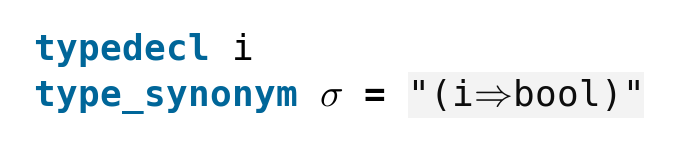
\includegraphics[width=0.4\textwidth]{resources/ShallowPrimTypes}
	\caption{World and Proposition types in shallow embedding}
	\end{figure}
In the developed deep embedding, both the worlds and propositions are elements of primitive types: the type of worlds $\mathcal{w}$ and the type of atomic propositions $\mathcal{P}$. 
	\begin{figure}
	\centering
	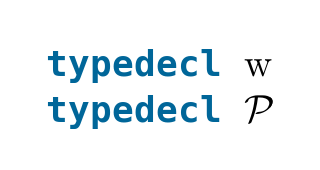
\includegraphics[width=0.2\textwidth]{resources/DeepPrimTypes}
	\caption{World and Proposition types in deep embedding}
	\end{figure}
The main difference is that in the shallow embedding, the evaluation of truthfulness is embedded within the propositions, as it is a map, whereas in deep approach the proposition is defined independently from its evaluation. To evaluate the proposition, the valuation function will be used. However this raises the question: if there might be different valuation of the same proposition, then show is shallow embedding deals with it? After all, a proposition is a map, just as the valuation. The answer is that in shallow embedding, such pairs of propositions and its evaluations will be different maps. Thus for a proposition $\varphi$ there will exist a family of functions $\lbrace \varphi_V \rbrace$ that represent the proposition under evaluation. This does not impact the definition of validity, but it does make difficult to reason about the details of the logic, as the formal definition of semantics treats propositions separate from their valuations.

In addition, we define the type of relations for both embeddings. For deep embedding we also define a type of characteristic sets of worlds and the type of valuations on a proposition in a given world.
	\begin{figure}[h]
	\centering
	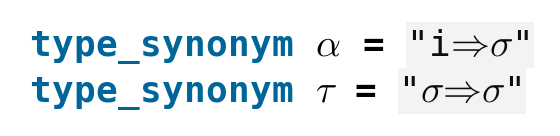
\includegraphics[width=0.3\textwidth]{resources/ShallowPrimTypesPt2}
	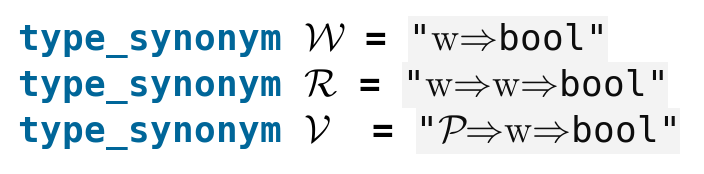
\includegraphics[width=0.3\textwidth]{resources/DeepPrimTypesPt2}
	\caption{Auxiliary types of relation, world set and valuation function}
	\end{figure}

\subsection{Embedding of syntax}
Given the type of propositions as maps, in shallow embedding, the deontic connectives are also constructed to be maps from worlds to boolean. The classical connectives like conjunction ($\land$), disjunction ($\lor$), negation ($\neg$) and implication ($\to$) are embedded as a wrapper around HOL connectives. The deontic elements $\square$ and $\circ$ are embedded using HOL logic, as functions from propositions to propositions. 
	\begin{figure}
	\centering
	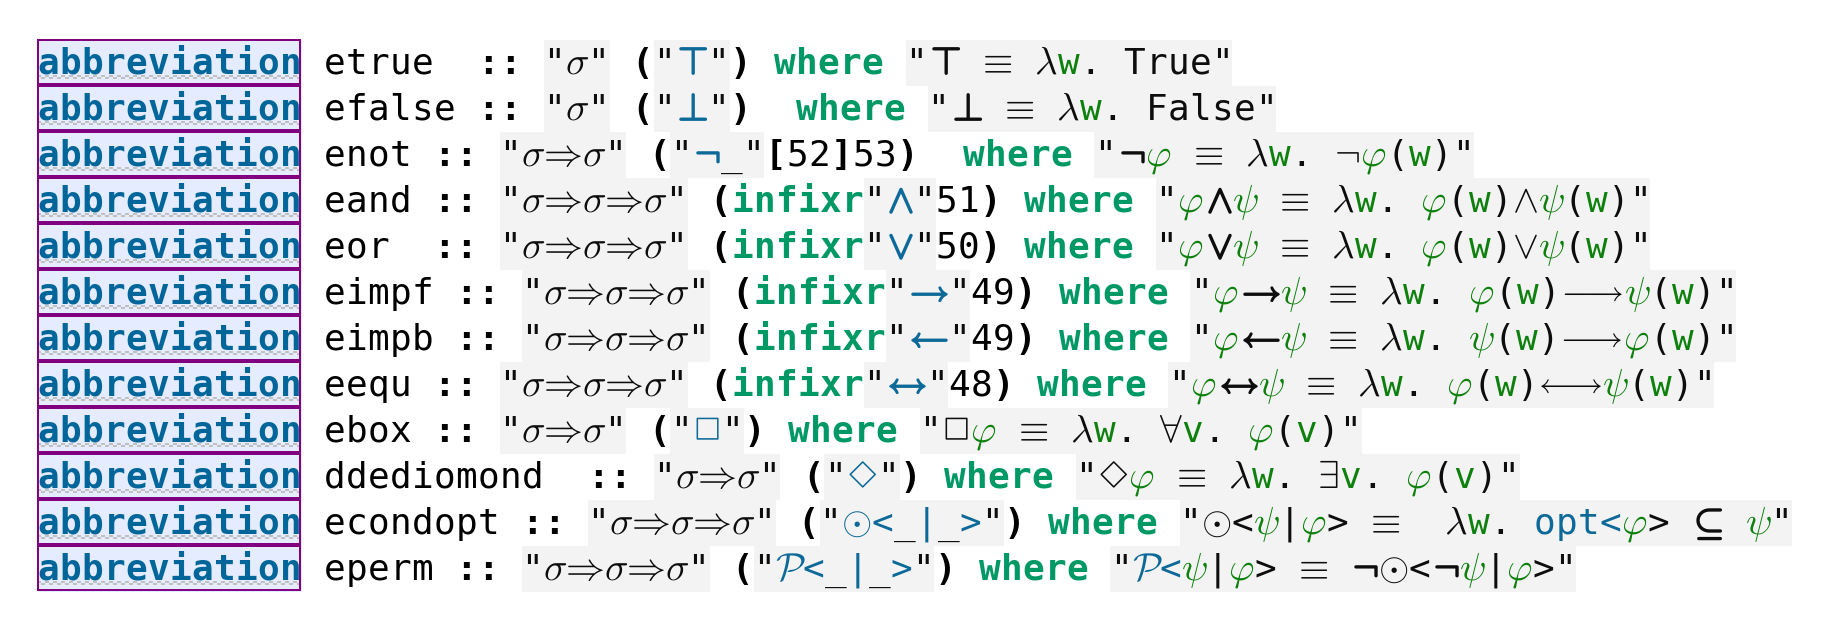
\includegraphics[width=0.5\textwidth]{resources/ShallowSyntaxFull}
	\caption{The syntax in shallow embedding}
	\end{figure}

In the deep embedding the syntax definition mimics the formal structure, defining the basic logical connectives and atomic formulas as constructors in a datatype \texttt{DDL}. Datatype in Isabelle define a new type, elements of which are formed by a finite application of constructors. In other words, the elements of the datatype are the least type closed under relations given by contructors. 
	\begin{figure}[h]
	\centering
	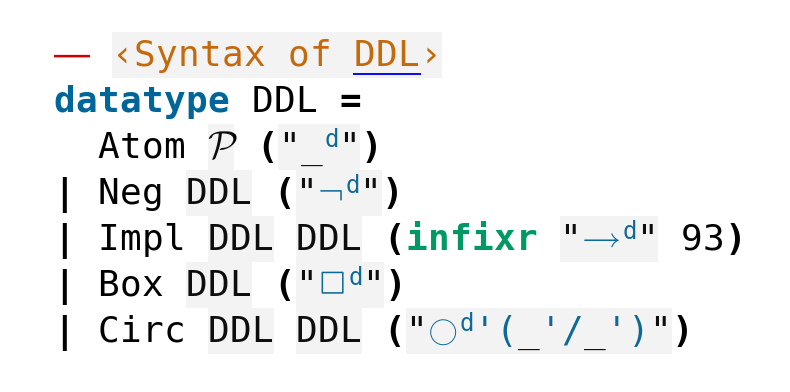
\includegraphics[width=0.34\textwidth]{resources/DeepSyntax}
	\caption{The syntax of DDL as a datatype definition. A DDL formula is an element of the \texttt{DDL} type}
	\end{figure}

\subsection{Embedding of semantics}
The embedding of semantics differs drastically in shallow and deep embedding. In shallow, the semantics is embedded into the syntax definition, as the syntax provides also the satisfiability operation. The validity then is as simple, as requiring that all propositions are valid for all worlds. Here, propositions already contain the relation and valuation in them. 
	\begin{figure}[h]
	\centering
	
\includegraphics[width=0.5\textwidth]{resources/ShallowValidity}
	\caption{Validity in shallow embedding}
	\end{figure}

My approach was inspired by the deep embedding of propositional logic in \cite{Benz}, to define the satisfiability of a formula as a primitive recursion (function) that evaluates a formula given a model and a world. 
	\begin{figure}[h]
	\centering
	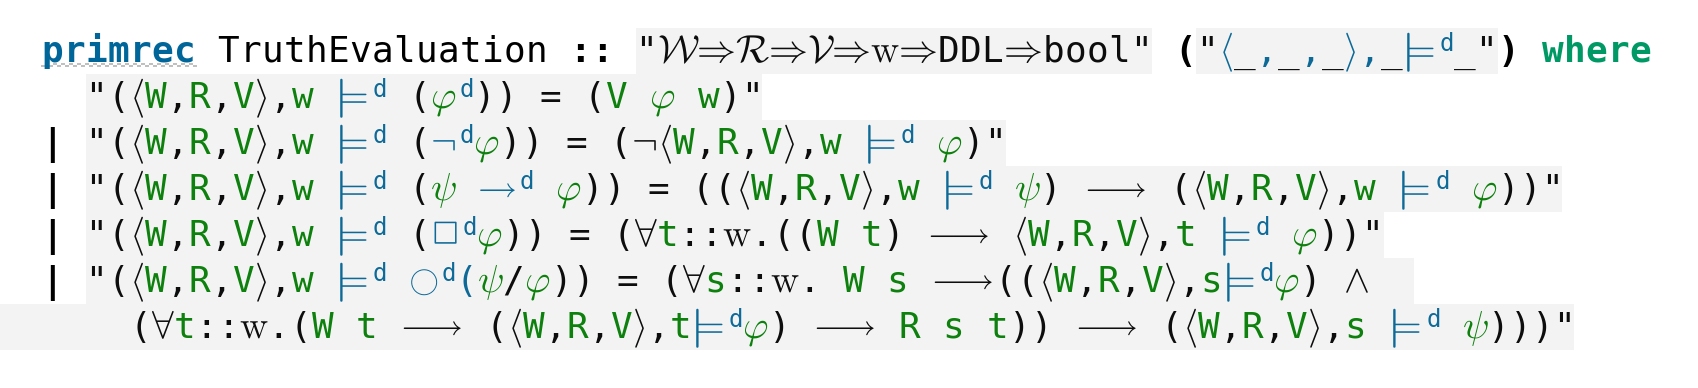
\includegraphics[width=0.5\textwidth]{resources/DeepSat}
	\caption{Satisfiability in deep embedding}
	\end{figure}

Note that in both shallow and deep, the optimality condition is used. While embedding of Parent and Benzmüller does consider both the optimal and maximal versions of best states, I have not done the satisfiability for maximal notion.

For the validity, all worlds must satisfy a formula quantified over all models with reflexive, transitive and total relations.
	\begin{figure}[h]
	\centering
	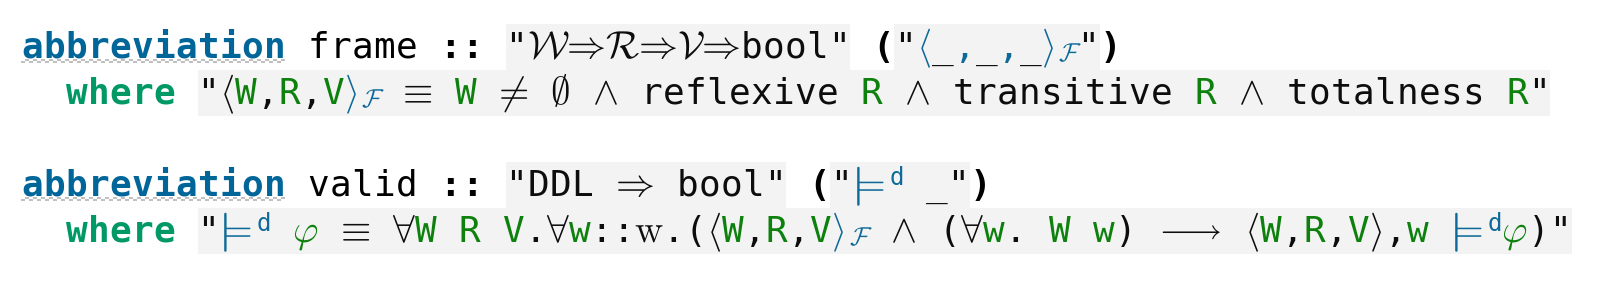
\includegraphics[width=0.5\textwidth]{resources/DeepValidity}
	\caption{Validity in deep embedding}
	\end{figure}

\subsection{Embedding of proof system}
The proof system is where I took a different approach from embedding of Parent and Benzmüller. In their embedding, the proof system is not formalised as a definition or a structure, but rather is proved to be inside the semantics, given relation conditions. 
	\begin{figure}[h]
	\centering
	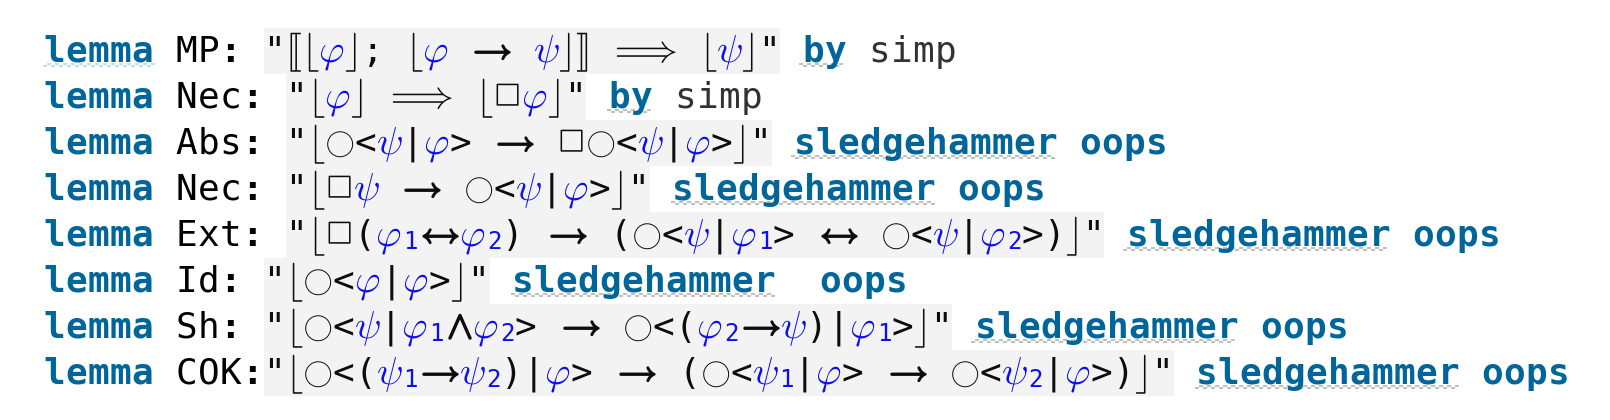
\includegraphics[width=0.5\textwidth]{resources/ShallowProofSystem}
	\caption{The lemmas that represent axiom and rule schemas in the Aqvist's proof system E }
	\end{figure}

	\begin{figure}[h]
	\centering
	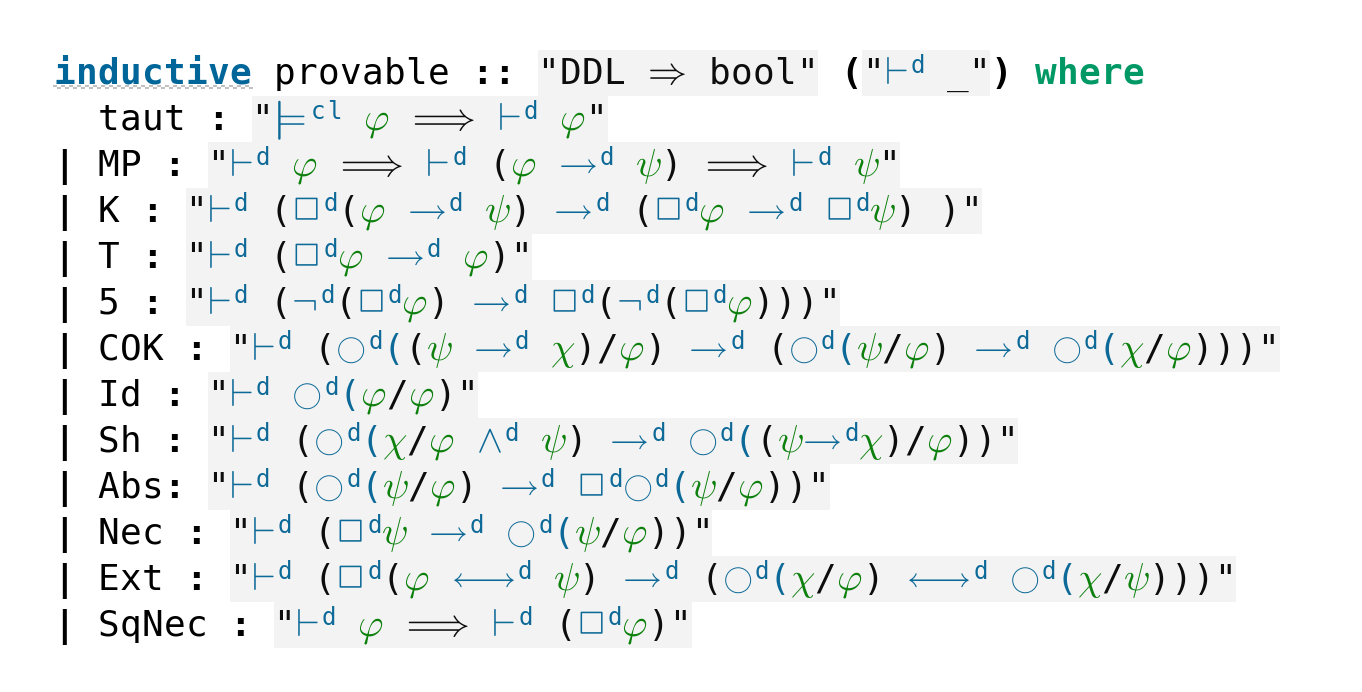
\includegraphics[width=0.5\textwidth]{resources/DeepProofSystem}
	\caption{The inductive definition defines a subset of formulas that can be "build" from axiom schemas using modus ponens (MP) and necessitation rule (SqNec)}
	\end{figure}
In my deep embedding, I have formalised Aqvist's proof system E as an inductive definition. An inductive definition is a least set closed under given relations. In case of the \texttt{provable} definition, it defines a characteristic function of a subset whose formulas can be constructed from the axiom schemas via a finite application of modus ponens and the necessitation rule schemas.

The proof that the semantics contains the proof system E is done in the soundness proof (see next section). Using the inductive definition, allows for a programming style notation of provability. Given a formula, in shallow embedding, checking if it is a provable formula required usage of sledgehammer or nitpick to show the statement. Using inductive definition automatically checks if a formula is provable. 

Inductive definitions are defined by constructing a monotone function on the powerset of formulas, whose fixed point is the least set closed under relations (using set theoretic language, in case of HOL a monotone lambda abstraction is used ), see \cite{inductdef}. Given a language, in which set theory is embedded, the inductive definition can also be implemented. This means that the developed proof system can be embedded in a language like Elixir, given an implementation of inductive definitions in Elixir.

The proof system E contains every classical tautology as the axiom schema. I have implemented it as a rule schema, where every classically valid formula ($\vDash^\text{cl}$) counts as a provable formula. 
	\begin{figure}[h]
	\centering
	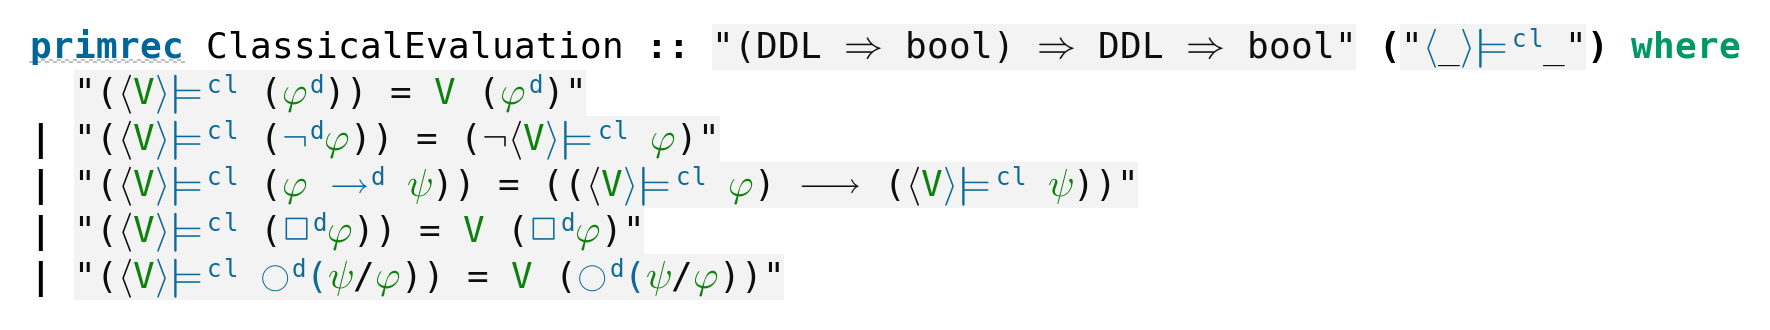
\includegraphics[width=0.5\textwidth]{resources/ClassicalSat}
	\caption{The classical satisfaction of a deontic formula}
	\end{figure}

	\begin{figure}[h]
	\centering
	
\includegraphics[width=0.5\textwidth]{resources/ClassicalValidity}
	\caption{Classical validity}
	\end{figure}
The classical evaluation of deontic formulas $\square \varphi$ and $\bigcirc(\phi/ \varphi)$ treats them as just atomic classical proposition. The valuation function must assign them truth or falsehood.

\section{Proof of soundness}
The definition of soundness is that any provable formula within the proof system is valid in the semantics, i.e.
$$\vdash \varphi \Longrightarrow \vDash \varphi$$
The proof of soundness also shows that given the semantics with preference models where the relation is reflexive, transitive and total correspond to axioms in the proof system.
\subsection{Overview of the proof}
The proof is by structural induction on \texttt{provable} definition. Most cases are solved by simplification, and evaluation of the axiom schema. The special case is showing that classical tautologies are valid in DDL semantics.
\subsection{The bridge lemma}
To show that classical tautology is also valid, we show that the deontic evaluation function can be used as a classical valuation function. This is done by fixing the model and a world, and using the resulting partial function as the classical valuation. 
	\begin{figure}[h]
	\centering
	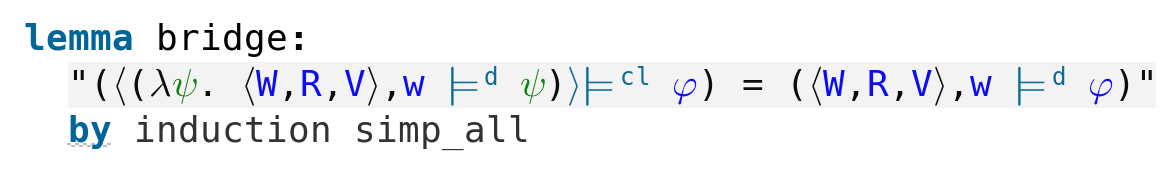
\includegraphics[width=0.5\textwidth]{resources/BridgeLemma}
	\caption{The inductive definition defines a subset of formulas that can be "build" from axiom schemas using modus ponens (MP) and necessitation rule (SqNec)}
	\end{figure}
Using the bridge lemma, proving that classical validity implies deontic valitidy is done by induction on the classical validity and using bridge lemma to simplify it.

\section{Conclusion}
I have developed a deep embedding of dyadic deontic logic within Isabelle/HOL and Aqvist's proof system E. The proof system is sound for semantics with class of all preference models and for the class of models with reflexive, transitive and total relation. The developed embedding can be used within the LogiKEY methodology, for mechanisation of conditional normative reasoning. The style of deep embedding is closer to that of usual purely functional programming languages, thus the deep embedding can be ported to other functional languages, such as Elixir, for practical use in embedded systems. Another further development might be porting the embedding to the Lean programming language and proof assistant. Despite being known for its use in the field of formalising mathematical proofs, Lean 4 was developed to be a pure functional general purpose programming language. Its efficiency, as well as style of coding is that of the Haskell programming language. Porting the embedding to Lean would combine both the automatic reasoner and programming language compiler to produce an executable. Future developments are to show completeness of the system, show correspondence between the properties of the relation in the preference model and axiom schemas in the proof system.


\begin{thebibliography}{9}
\bibitem{LogiKey} Designing Normative Theories for Ethical and Legal Reasoning: LogiKEy Framework, Methodology, and Tool Support. Benzmüller C., Parent X., \& van der Torre L., Artificial Intelligence, 287: 103348. 2020.
\bibitem{Benz} Faithful Logic Embeddings in HOL — Deep and Shallow. Benzmüller, C. In Barrett, C., \& Waldmann, U., editor(s), Automated Deduction – CADE-30 – 30th International Conference on Automated Deduction, Stuttgart, Germany, July 28-31, 2025, Proceedings, volume 15943, of Lecture Notes in Computer Science, pages 280–302, 2025. Springer
\bibitem{book} Introduction to Deontic Logic and Normative Systems https://www.collegepublications.co.uk/downloads/TLR00001.pdf
\bibitem{shallow} Normative Conditional Reasoning as a Fragment of HOL. Xavier Parent, Christoph Benzmüller arXiv:2308.10686
\bibitem{inductdef} Gordon Plotkin; Colin P. Stirling; Mads Tofte, "A Fixedpoint Approach to (Co)Inductive and (Co)Datatype Definitions," in Proof, Language, and Interaction: Essays in Honour of Robin Milner , MIT Press, 2000, pp.187-211.
\end{thebibliography}

\end{document}

